\documentclass[aspectratio=169,11pt]{beamer}
\usepackage[T1]{fontenc}
\usepackage{lmodern}
\usepackage{amsmath,amssymb,booktabs}
\usepackage{tikz}
\usetikzlibrary{arrows.meta,positioning,calc,decorations.pathreplacing}

\definecolor{ink}{HTML}{172A3A}
\definecolor{teal}{HTML}{008B80}
\definecolor{amber}{HTML}{BF761C}
\definecolor{muted}{HTML}{526574}
\definecolor{pale}{HTML}{EAF5F3}
\definecolor{papergray}{HTML}{F2F5F7}
\setbeamercolor{normal text}{fg=ink,bg=white}
\setbeamercolor{structure}{fg=teal}
\setbeamercolor{frametitle}{fg=ink}
\setbeamercolor{block title}{fg=teal,bg=pale}
\setbeamercolor{block body}{fg=ink,bg=pale}
\setbeamercolor{takeaway}{fg=ink,bg=pale}
\setbeamercolor{footline}{fg=muted,bg=white}
\setbeamerfont{frametitle}{size=\Large,series=\bfseries}
\setbeamerfont{framesubtitle}{size=\small}
\setbeamerfont{block title}{series=\bfseries}
\setbeamerfont{footline}{size=\tiny}
\setbeamertemplate{navigation symbols}{}
\setbeamertemplate{itemize item}{\small\raisebox{0.1ex}{$\bullet$}}
\setbeamertemplate{bibliography item}[text]
\setbeamersize{text margin left=9mm,text margin right=9mm}
\setbeamertemplate{footline}{%
  \begin{beamercolorbox}[wd=\paperwidth,ht=3.5ex,dp=1.5ex,leftskip=9mm,rightskip=9mm]{footline}
  Przemysław Uznański\hfill Rectangular matrix multiplication\hfill
  \insertframenumber\,/\,\inserttotalframenumber
  \end{beamercolorbox}}
\hypersetup{colorlinks=true,urlcolor=teal,linkcolor=teal,citecolor=teal,
  pdftitle={Rectangular matrix multiplication from polynomial products},
  pdfauthor={Przemysław Uznański}}

\newcommand{\CC}{\mathbb C}
\newcommand{\rank}{\operatorname{rank}}
\newcommand{\degen}{\unrhd}
\newcommand{\cmm}[3]{\langle #1,#2,#3\rangle}
\newcommand{\source}[1]{\vfill\par{\fontsize{7.5}{9}\selectfont\color{muted}#1\par}}
\newcommand{\takeaway}[1]{\begin{beamercolorbox}[sep=0.65em,wd=\linewidth]{takeaway}#1\end{beamercolorbox}}
\newcommand{\doi}[1]{\href{https://doi.org/#1}{\nolinkurl{#1}}}
\tikzset{flow/.style={draw=teal!60,fill=pale,rounded corners=2pt,
  align=center,minimum height=9mm,font=\small},
  arrow/.style={-{Latex[length=2mm]},thick,teal},
  matrix/.style={draw=teal,fill=teal!12,thick}}

\title{Rectangular matrix multiplication\\from polynomial products}
\author{Przemysław Uznański}
\institute{Pathway}
\date{Preliminary slides \textbullet\ October 2026}

\begin{document}

% 1. Title.
\begin{frame}[plain]
  \vspace{5mm}
  {\color{teal}\rule{20mm}{1.4mm}}\par\vspace{4mm}
  {\fontsize{26}{31}\selectfont\bfseries Rectangular matrix multiplication\\
  from polynomial products\par}
  \vspace{8mm}
  {\large Przemysław Uznański}\par\vspace{1mm}
  Pathway \quad\href{mailto:przemek@pathway.com}{\texttt{przemek@pathway.com}}
  \vspace{6mm}
  \takeaway{How far can the methods behind the bound $\omega\le2.25$\newline
  be pushed for rectangular products?}
  \vfill
  {\small Preliminary slides \textbullet\ October 2026}\par\vspace{2mm}
  {\fontsize{8}{10}\selectfont\color{muted}
  Based on the accompanying note. Slides prepared with GPT-6.1.\par}
\end{frame}

% 2. Square exponent: introduce the computational question before rectangles.
\begin{frame}{What is $\omega$?}
  Given $A,B\in\CC^{n\times n}$, compute $C=AB$ exactly.
  \begin{block}{The matrix-multiplication exponent}
    $\omega$ is the infimum of exponents $\tau$ for which some algorithm
    multiplies two $n\times n$ matrices using $O(n^\tau)$ field operations.
  \end{block}
  \medskip
  \begin{columns}[T,onlytextwidth]
    \begin{column}{0.47\textwidth}
      \textbf{The usual algorithm}\par\medskip
      $n^2$ dot products of length $n$:
      \[
        O(n^3),\qquad\omega\le3.
      \]
    \end{column}
    \begin{column}{0.47\textwidth}
      \textbf{Strassen's algorithm}\par\medskip
      Seven recursive products of half-size blocks:
      \[
        O(n^{\log_2 7}),\qquad\omega\le\log_2 7\approx2.80735.
      \]
    \end{column}
  \end{columns}
  \takeaway{There are $n^2$ outputs, so $\omega\ge2$.
    The central open question is whether $\omega=2$.}
  \source{We count field operations over $\CC$, as in the note.
  Throughout, $O(n^e)$ suppresses a $+o(1)$ term in the exponent.
  Strassen: \href{https://doi.org/10.1007/BF02165411}{Gaussian elimination is not optimal (1969)}.}
\end{frame}

% 3. Selected square milestones; links point to the original papers.
\begin{frame}{A short history of square matrix multiplication}
  \begin{center}
  \small
  \renewcommand{\arraystretch}{1.22}
  \begin{tabular}{@{}lll@{}}
    \toprule
    Year & Algorithm / analysis & Upper bound on $\omega$\\
    \midrule
    Classical & Entry-by-entry dot products & $3$\\
    1969 & \href{https://doi.org/10.1007/BF02165411}{Strassen} & $\log_2 7\approx2.80735$\\
    1990 & \href{https://doi.org/10.1016/0747-7171(90)90013-2}{Coppersmith--Winograd} & $2.375477$\\
    2014 & \href{https://arxiv.org/abs/1401.7714}{Le Gall} & $2.3728639$\\
    2024 & \href{https://arxiv.org/abs/2404.16349}{Alman et al.} & $2.371339$\\
    Aug.\ 2026 & \href{https://arxiv.org/abs/2608.16884}{Dupont et al.}: optimization + AlphaEvolve & $2.371177$\\
    Sept.\ 2026 & \href{https://github.com/openai/math/tree/main/preprints/Complex-Matrix-Multiplication-Below-2.258-and-Rectangular-Bounds-September-24-2026}{Polynomial-product / completion analysis} & $2.258$\\
    Oct.\ 2026 & Polynomial-product bound~\cite{nine-fourths} & $2.25$\\
    \bottomrule
  \end{tabular}
  \end{center}
  \medskip
  \takeaway{This talk asks how the methods behind the $2.25$ bound
    extend to rectangular products.}
\end{frame}

% 4. General shapes and the matching matrix dimensions.
\begin{frame}{What is $\omega(a,b,c)$?}
  For fixed $a,b,c\ge0$, consider the product
  \[
    (n^a\times n^b)\ \cdot\ (n^b\times n^c)
    \quad\longrightarrow\quad(n^a\times n^c).
  \]
  Its infimum running-time exponent is $\boldsymbol{\omega(a,b,c)}$.
  \medskip
  \begin{center}
  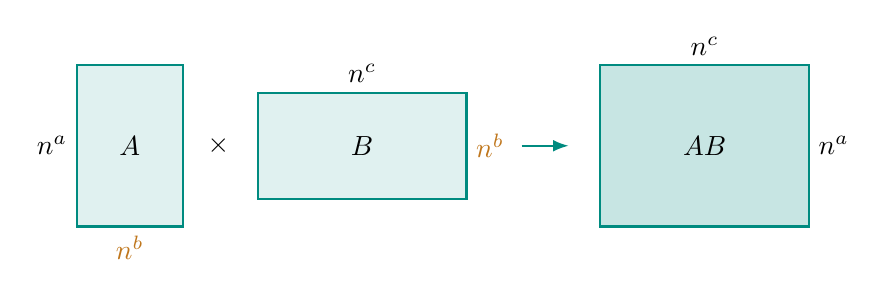
\begin{tikzpicture}[x=1cm,y=1cm]
    \draw[matrix] (0,0) rectangle (1.35,2.05);
    \node at (0.675,1.025) {$A$};
    \node[left] at (0,1.025) {$n^a$};
    \node[below,text=amber] at (0.675,0) {$n^b$};
    \node at (1.8,1.025) {$\times$};
    \draw[matrix] (2.3,0.35) rectangle (4.95,1.7);
    \node at (3.625,1.025) {$B$};
    \node[above] at (3.625,1.7) {$n^c$};
    \node[right,text=amber] at (4.95,1.025) {$n^b$};
    \draw[arrow] (5.65,1.025) -- (6.25,1.025);
    \draw[matrix,fill=teal!22] (6.65,0) rectangle (9.3,2.05);
    \node at (7.975,1.025) {$AB$};
    \node[above] at (7.975,2.05) {$n^c$};
    \node[right] at (9.3,1.025) {$n^a$};
  \end{tikzpicture}
  \end{center}
  \source{Exact multiplication over $\CC$; dimensions are rounded upward.}
\end{frame}

% 5. The usual one-parameter curve, its dual exponent, and their history.
\begin{frame}{The rectangular curve and the dual exponent}
  \begin{columns}[T,onlytextwidth]
    \begin{column}{0.43\textwidth}
      \textbf{Two useful special parameters}
      \[
        \omega(k)=\omega(1,k,1),\qquad\omega(1)=\omega.
      \]
      \[
        \alpha=\sup\{k\ge0:\omega(k)=2\}.
      \]
      The \textbf{dual exponent} $\alpha$ measures how far quadratic-time
      multiplication reaches as the inner dimension grows.
    \end{column}
    \begin{column}{0.53\textwidth}
      \textbf{Rectangular milestones}\par\smallskip
      {\footnotesize
      \setlength{\tabcolsep}{3pt}
      \renewcommand{\arraystretch}{1.15}
      \begin{tabular}{@{}lll@{}}
        \toprule
        Year & Source & Bound on $\alpha$\\
        \midrule
        1997 & \href{https://doi.org/10.1006/jcom.1997.0438}{Coppersmith} & $>0.29462$\\
        2012 & \href{https://arxiv.org/abs/1204.1111}{Le Gall} & $>0.30298$\\
        2018 & \href{https://arxiv.org/abs/1708.05622}{Le Gall--Urrutia} & $>0.31389$\\
        2024 & \href{https://arxiv.org/abs/2307.07970}{Vassilevska Williams et al.} & $\ge0.321334$\\
        Sept.\ 2026 & \href{https://github.com/openai/math/tree/main/preprints/Complex-Matrix-Multiplication-Below-2.258-and-Rectangular-Bounds-September-24-2026}{OpenAI preprint} & $>0.465$\\
        \textbf{This note} & \textbf{Rectangular extension} & $\boldsymbol{\ge0.5}$\\
        \bottomrule
      \end{tabular}}
    \end{column}
  \end{columns}
  \medskip
  \takeaway{Motivation: extend the polynomial-product analysis in~\cite{nine-fourths}
  to the shapes used by all-pairs algorithms, and make the proof accessible to TCS.}
  \source{These works also bound the curve $\omega(k)$ beyond the quadratic range;
  $\alpha$ summarizes where that range ends.
  Dimensions are rounded upward.}
\end{frame}

% 6. Theorem 1.1 (cor:general-exponents).
\begin{frame}{A bound for every matrix shape}
  Sort the three exponents: $a\ge b\ge c\ge0$.
  \begin{block}{Theorem 1.1 of the note}
  \[
    \omega(a,b,c)\le
    \begin{cases}
      a+b,&c\le\dfrac{ab}{a+b},\\[5pt]
      \dfrac{a+b+c}{2}
      +\dfrac{1}{4}\!\left(\dfrac{ab}{c}+\dfrac{ac}{b}+\dfrac{bc}{a}\right),
      &c>\dfrac{ab}{a+b}.
    \end{cases}
  \]
  \end{block}
  \medskip
  \takeaway{If $c\le\frac{ab}{a+b}$, the exponent is exactly $a+b$.}
  \medskip
  Permuting tensor legs lets us use the sorted dimensions of any product.
  \source{The largest input size supplies the lower bound $a+b$.}
\end{frame}

% 7. Corollary 1.2 (thm:curve).
\begin{frame}{The rectangular curve}
  \begin{block}{Corollary 1.2 of the note}
  \[
    \omega(k)\le
    \begin{cases}
      2,&0\le k\le\frac{1}{2},\\[3pt]
      1+k+\dfrac{1}{4k},&k\ge\frac{1}{2}.
    \end{cases}
  \]
  \end{block}
  \vspace{2mm}
  \begin{columns}[T,onlytextwidth]
    \begin{column}{0.47\textwidth}
      \textbf{The thin range is exact.}\par\medskip
      $\omega(k)=2$ for $0\le k\le\frac{1}{2}$.\par\medskip
      The dual exponent satisfies $\alpha\ge\frac{1}{2}$.
    \end{column}
    \begin{column}{0.47\textwidth}
      \textbf{Selected values.}\par\medskip
      \begin{tabular}{@{}ccc@{}}
      $k$ & $1$ & $2$\\
      \midrule
      $\omega(k)\le$ & $2.25$ & $3.125$
      \end{tabular}\par\medskip
      For $k\ge1$, the gap above the size lower bound is at most $\frac{1}{4k}$.
    \end{column}
  \end{columns}
  \source{$\alpha=\sup\{k\ge0:\omega(k)=2\}$.
  The lower bound is $\omega(k)\ge\max\{2,1+k\}$.}
\end{frame}

% 8. Reuse the manuscript's vector figure.
\begin{frame}{The bound for $0\le k\le2$}
  \centering
  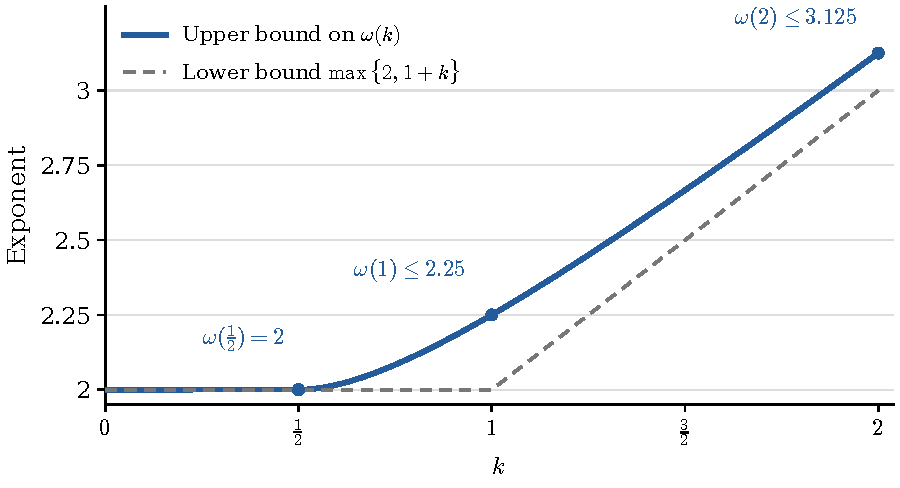
\includegraphics[width=0.88\textwidth,height=0.73\textheight,keepaspectratio]{../rectangular-exponent-curve.pdf}
  \par\vspace{2mm}
  \takeaway{For $0\le k\le\frac{1}{2}$, the upper bound meets the size lower bound.}
\end{frame}

% 9. Interfaces between the four parts of the proof.
\begin{frame}{The proof in four steps}
  \begin{center}
  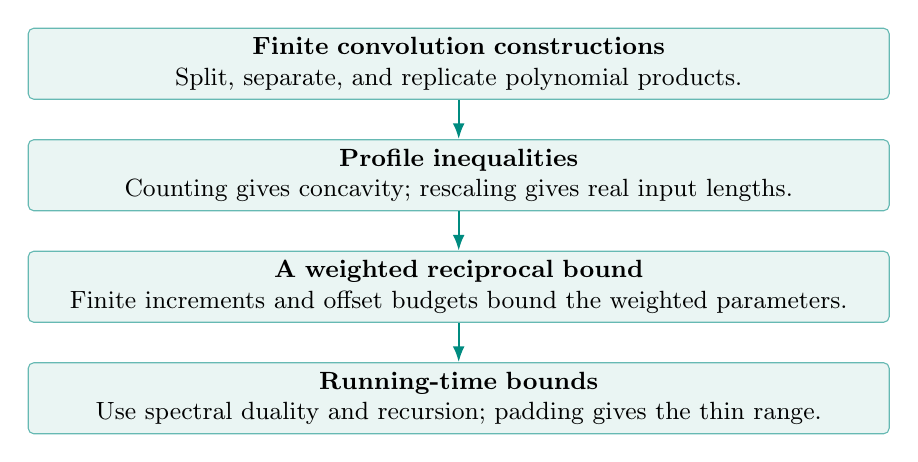
\begin{tikzpicture}[node distance=5mm]
    \node[flow,text width=10.7cm] (a) {\textbf{Finite convolution constructions}\\
      Split, separate, and replicate polynomial products.};
    \node[flow,text width=10.7cm,below=of a] (b) {\textbf{Profile inequalities}\\
      Counting gives concavity; rescaling gives real input lengths.};
    \node[flow,text width=10.7cm,below=of b] (c) {\textbf{A weighted reciprocal bound}\\
      Finite increments and offset budgets bound the weighted parameters.};
    \node[flow,text width=10.7cm,below=of c] (d) {\textbf{Running-time bounds}\\
      Use spectral duality and recursion; padding gives the thin range.};
    \draw[arrow] (a) -- (b); \draw[arrow] (b) -- (c); \draw[arrow] (c) -- (d);
  \end{tikzpicture}
  \end{center}
  \source{Sections 2--6 of the note. The spectral theorem is a published input;
  the rectangular parameter analysis is the extension studied here.}
\end{frame}

% Toolkit 1. Establish the ordinary computation and the allowed algorithm shape.
\begin{frame}{Ordinary block multiplication uses eight products}
  \[
    A=\begin{pmatrix}a_{11}&a_{12}\\a_{21}&a_{22}\end{pmatrix},\qquad
    B=\begin{pmatrix}b_{11}&b_{12}\\b_{21}&b_{22}\end{pmatrix},\qquad C=AB.
  \]
  \begin{columns}[T,onlytextwidth]
    \begin{column}{0.47\textwidth}
      \textbf{Four outputs, two products each}
      \[
      \begin{aligned}
        c_{11}&=a_{11}b_{11}+a_{12}b_{21},\\
        c_{12}&=a_{11}b_{12}+a_{12}b_{22},\\
        c_{21}&=a_{21}b_{11}+a_{22}b_{21},\\
        c_{22}&=a_{21}b_{12}+a_{22}b_{22}.
      \end{aligned}
      \]
    \end{column}
    \begin{column}{0.49\textwidth}
      \textbf{We may use linear combinations}
      \begin{enumerate}
        \item Add or subtract blocks within each input.
        \item Multiply one combination from each input.
        \item Add or subtract the products to form the outputs.
      \end{enumerate}
    \end{column}
  \end{columns}
  \medskip
  \takeaway{Can linear combinations reduce the eight multiplications?}
  \source{The entries $a_{ij}$ and $b_{ij}$ may be scalars or matrix blocks.
  Ordinary block recursion gives $T(n)=8T(n/2)+O(n^2)$, including all additions.}
\end{frame}

% Toolkit 2. All seven products and the exact output recombinations.
\begin{frame}{Strassen's seven products and four outputs}
  For the same matrices $A$ and $B$, compute $C=AB$ as follows.
  \medskip
  \begin{columns}[T,onlytextwidth]
    \begin{column}{0.45\textwidth}
      \textbf{Compute these seven products}
      \[
      \begin{aligned}
        M_1&=(a_{11}+a_{22})(b_{11}+b_{22}),\\
        M_2&=(a_{21}+a_{22})b_{11},\\
        M_3&=a_{11}(b_{12}-b_{22}),\\
        M_4&=a_{22}(b_{21}-b_{11}),\\
        M_5&=(a_{11}+a_{12})b_{22},\\
        M_6&=(a_{21}-a_{11})(b_{11}+b_{12}),\\
        M_7&=(a_{12}-a_{22})(b_{21}+b_{22}).
      \end{aligned}
      \]
    \end{column}
    \begin{column}{0.52\textwidth}
      \textbf{Add and subtract to get the outputs}
      \[
      \begin{aligned}
        c_{11}&=M_1+M_4-M_5+M_7,\\
        c_{12}&=M_3+M_5,\\
        c_{21}&=M_2+M_4,\\
        c_{22}&=M_1-M_2+M_3+M_6.
      \end{aligned}
      \]
      For example, the first combination simplifies to
      $c_{11}=a_{11}b_{11}+a_{12}b_{21}$.
    \end{column}
  \end{columns}
  \takeaway{Seven block products give
    $\displaystyle T(n)=7T(n/2)+O(n^2)$, hence $\omega\le\log_2 7$.}
  \source{Strassen (1969):
  \href{https://doi.org/10.1007/BF02165411}{Gaussian elimination is not optimal}.
  Every product has a left-input factor followed by a right-input factor;
  the same formulas therefore apply to matrix blocks.}
\end{frame}

% Toolkit 3. The full equality of the eight-term and seven-term decompositions.
\begin{frame}{Tensor rank counts bilinear products}
  Use formal labels $c_{ij}$ for the four output positions:
  \[
    T=\underbrace{
      \begin{aligned}
        &a_{11}b_{11}c_{11}+a_{12}b_{21}c_{11}
          +a_{11}b_{12}c_{12}+a_{12}b_{22}c_{12}\\
        &+a_{21}b_{11}c_{21}+a_{22}b_{21}c_{21}
          +a_{21}b_{12}c_{22}+a_{22}b_{22}c_{22}
      \end{aligned}
    }_{\text{8 ordinary terms}}
  \]
  \[
  \begin{aligned}
    ={}&(a_{11}+a_{22})(b_{11}+b_{22})(c_{11}+c_{22})\\
       &+(a_{21}+a_{22})b_{11}(c_{21}-c_{22})
         +a_{11}(b_{12}-b_{22})(c_{12}+c_{22})\\
       &+a_{22}(b_{21}-b_{11})(c_{11}+c_{21})
         +(a_{11}+a_{12})b_{22}(c_{12}-c_{11})\\
       &+(a_{21}-a_{11})(b_{11}+b_{12})c_{22}
         +(a_{12}-a_{22})(b_{21}+b_{22})c_{11}.
  \end{aligned}
  \]
  \textbf{7 Strassen terms:} one linear form from each \textbf{leg} $a,b,c$.
  \takeaway{Tensor rank is the fewest such terms in a sum for $T$.
    This identity gives $\rank(\cmm{2}{2}{2})\le7$.}
  \source{Section 2. Collect each $M_r$'s coefficients in the four output formulas
  to obtain its linear form in $c$. For instance, $M_2$ multiplies $c_{21}-c_{22}$.}
\end{frame}

% Toolkit 4. Generalize the example and connect tensor rank to the exponent.
\begin{frame}{Matrix multiplication tensors and the exponent}
  All earlier improvements to $\omega$ fit this \textbf{Strassen-type bilinear
  framework}, including tensor powers and degenerations.
  \par\medskip
  \[
    \cmm{m}{r}{p}
    =\sum_{i=1}^{m}\sum_{k=1}^{r}\sum_{j=1}^{p}
      a_{ik}b_{kj}c_{ij}.
  \]
  It encodes $m\times r$ by $r\times p$ multiplication;
  $c_{ij}$ labels output position $(i,j)$.
  \par\medskip
  A rank-$R$ identity gives an algorithm using $R$ bilinear products.
  Applying a square identity with fixed block size $q$ recursively gives
  \[
    T(n)\le R\,T(n/q)+O(n^2).
  \]
  \takeaway{$\displaystyle
    \rank(\cmm{q}{q}{q})\le R
    \quad\Longrightarrow\quad \omega\le\log_q R.
  $}
  \source{Linear-map costs are
  included; the exponent convention absorbs logarithmic factors.}
\end{frame}

% Toolkit 5. Restriction: explicit input encoding and output decoding.
\begin{frame}{Restriction: reuse an algorithm after linear substitutions}
  Make linear substitutions independently on the $a$-, $b$-, and $c$-legs.
  \par\medskip
  \begin{columns}[T,onlytextwidth]
    \begin{column}{0.45\textwidth}
      \textbf{What happens to the algorithm?}\par\smallskip
      Linearly encode the new inputs, run the old bilinear products,
      then linearly combine their outputs.
      \par\medskip
      Each product of three linear forms remains a product of three
      linear forms after substitution.
    \end{column}
    \begin{column}{0.51\textwidth}
      \textbf{Example: keep only the first row}\par\smallskip
      Set $a_{21}=a_{22}=0$ in $2\times2$ multiplication:
      \[
        \begin{pmatrix}a_{11}&a_{12}\\0&0\end{pmatrix}
        \begin{pmatrix}b_{11}&b_{12}\\b_{21}&b_{22}\end{pmatrix}
        =\begin{pmatrix}c_{11}&c_{12}\\0&0\end{pmatrix}.
      \]
      This computes a $1\times2$ row times a $2\times2$ matrix:
      \[
        \cmm{2}{2}{2}\ge\cmm{1}{2}{2}.
      \]
    \end{column}
  \end{columns}
  \medskip
  \takeaway{$\displaystyle T\ge S\quad\Longrightarrow\quad
    \rank(S)\le\rank(T).$}
  \source{Section 2. The notation $T\ge S$ means that $T$ restricts to $S$.
  Substitutions on the formal output labels specify the linear decoding
  of outputs. Here the zero second row lets us retain only $c_{11},c_{12}$.}
\end{frame}

% Toolkit 6. Direct sum: disjoint inputs and outputs, concatenated algorithms.
\begin{frame}{Direct sum: run independent computations side by side}
  Use disjoint variables on all three legs:
  \[
    T(a,b,c)\oplus U(a',b',c')=T(a,b,c)+U(a',b',c').
  \]
  \begin{columns}[T,onlytextwidth]
    \begin{column}{0.45\textwidth}
      \textbf{Example: two scalar products}\par\smallskip
      \[
        a_1b_1c_1+a_2b_2c_2
      \]
      encodes the two separate outputs
      \[
        c_1=a_1b_1,\qquad c_2=a_2b_2.
      \]
    \end{column}
    \begin{column}{0.51\textwidth}
      \textbf{How the algorithms combine}\par\smallskip
      If $T$ uses $R$ products and $U$ uses $S$ products,
      concatenate the lists: $R+S$ products compute both.
      \par\medskip
      We write $mT$ for $m$ independent copies of $T$,
      each with its own inputs and outputs.
    \end{column}
  \end{columns}
  \medskip
  \takeaway{$\displaystyle
    \rank(T\oplus U)\le\rank(T)+\rank(U).
  $}
\end{frame}

% Toolkit 7. Derive block composition and mention general rank submultiplicativity.
\begin{frame}{Why tensor products give block multiplication}
  Take $q\times q$ blocks, each an $s\times s$ matrix.
  \par\medskip
  \begin{columns}[T,onlytextwidth]
    \begin{column}{0.45\textwidth}
      {\centering
      \renewcommand{\arraystretch}{1.15}
      \begin{tabular}{@{}ccc@{}}
        \toprule
        Outer & Inner & Paired variable\\
        \midrule
        $a_{ik}$ & $a'_{uw}$ & $a_{(i,u),(k,w)}$\\
        $b_{kj}$ & $b'_{wv}$ & $b_{(k,w),(j,v)}$\\
        $c_{ij}$ & $c'_{uv}$ & $c_{(i,u),(j,v)}$\\
        \bottomrule
      \end{tabular}
      \par}
      \smallskip
      $(i,u)$ has $qs$ possible values.
    \end{column}
    \begin{column}{0.52\textwidth}
      The coefficient of $c_{(i,u),(j,v)}$ is
      \[
        \sum_{k=1}^{q}\sum_{w=1}^{s}
          a_{(i,u),(k,w)}\,b_{(k,w),(j,v)}.
      \]
      This is the usual row--column dot product over all $qs$ inner indices $(k,w)$.
    \end{column}
  \end{columns}
  \medskip
  \takeaway{$\displaystyle
    \cmm{q}{q}{q}\otimes\cmm{s}{s}{s}\cong\cmm{qs}{qs}{qs}.
    $\newline
    Iterating gives $\displaystyle
    \cmm{q}{q}{q}^{\otimes N}\cong\cmm{q^N}{q^N}{q^N}$.
  }
  \smallskip
  Pairing rank-one terms also gives
  $\rank(T\otimes S)\le\rank(T)\rank(S)$.
  \source{Paired variables are independent coordinates. Relabel
  $(i,u)\leftrightarrow(i-1)s+u$, and similarly for the column and inner indices.
  Expanding the two tensors gives the displayed output coefficient;
  $q,s,N$ are positive integers.}
\end{frame}

% Toolkit 8. Define degeneration before the interpolation argument.
\begin{frame}{Degeneration: a limit of restrictions}
  Fix tensors $T$ and $S$: $T$ is the available computation;
  $S$ is the desired computation.
  \begin{block}{Definition}
    A \textbf{degeneration} $T\degen S$ is a family of linear substitutions
    on the three legs of $T$, depending on $\varepsilon\ne0$, whose resulting
    tensors $P(\varepsilon)$ converge \textbf{coefficient by coefficient} to $S$
    as $\varepsilon\to0$.
  \end{block}
  \medskip
  \[
    T\ge P(\varepsilon)\quad(\varepsilon\ne0),
    \qquad \lim_{\varepsilon\to0}P(\varepsilon)=S.
  \]
  \medskip
  For every $a_i b_j c_k$, its coefficient in $P(\varepsilon)$ must tend
  to its coefficient in $S$.
  \source{Definition: Section 2 of the note. Substitutions act independently
  on the three legs; all $P(\varepsilon)$ use the same coordinates as $S$.}
\end{frame}

% Toolkit 9. Singular substitutions can reach beyond ordinary restriction.
\begin{frame}[label=degeneration-example]{A degeneration that cannot be a restriction}
  \textbf{Available:} $T=a'_0b'_0c'_0+a'_1b'_1c'_1$
  (two independent scalar products).
  \par\smallskip
  \textbf{Target:} $S=a_0b_0c_0+(a_0b_1+a_1b_0)c_1$.
  \par\medskip
  For $\varepsilon\ne0$, substitute independently on the three legs:
  \[
  \begin{array}{lll}
    a'_0\mapsto a_0,& b'_0\mapsto b_0,&
      c'_0\mapsto c_0-c_1/\varepsilon,\\[3pt]
    a'_1\mapsto a_0+\varepsilon a_1,&
      b'_1\mapsto b_0+\varepsilon b_1,&
      c'_1\mapsto c_1/\varepsilon.
  \end{array}
  \]
  \[
  \begin{aligned}
    P(\varepsilon)
      &=a_0b_0\left(c_0-\frac{c_1}{\varepsilon}\right)
        +(a_0+\varepsilon a_1)(b_0+\varepsilon b_1)\frac{c_1}{\varepsilon}\\
      &=S+\varepsilon a_1b_1c_1.
  \end{aligned}
  \]
  \takeaway{The substitutions contain $1/\varepsilon$ and are undefined at zero,
    but their divergent terms cancel: $P(\varepsilon)\to S$.\newline
    $T\degen S$, whereas $T\not\ge S$: $\rank(T)=2<3=\rank(S)$.}
  \source{All primed variables are independent. The target is the standard
  $W$-tensor with its output coordinates exchanged;
  see \cite[proof of Proposition 13, p.~131]{interpolation}.
  \hyperlink{degeneration-rank-proof}{Rank-three proof in backup.}}
\end{frame}

% Toolkit 10. Define asymptotic rank and justify its use for the exponent.
\begin{frame}{Asymptotic rank is enough to bound $\omega$}
  The \textbf{asymptotic rank} measures the growth of rank under tensor powers:
  \[
    \widetilde R(T):=\lim_{N\to\infty}\rank(T^{\otimes N})^{1/N}
      =\inf_{N\ge1}\rank(T^{\otimes N})^{1/N}.
  \]
  Fix an integer $q\ge2$ and put $M=\cmm{q}{q}{q}$.
  A rank decomposition of
  $M^{\otimes N}\cong\cmm{q^N}{q^N}{q^N}$ gives a block algorithm
  of side $q^N$. Recursing gives
  \[
    \omega\le\log_{q^N}\rank(M^{\otimes N})
      =\frac{\log_q\rank(M^{\otimes N})}{N}.
  \]
  \takeaway{Taking the infimum over $N$ gives the same conclusion as a rank bound:
    \[
      \widetilde R(\cmm{q}{q}{q})\le R
        \quad\Longrightarrow\quad\omega\le\log_q R.
    \]}
  \source{Definition: Section 3; algorithm conversion: Section 6.
  Submultiplicativity of rank ensures the limit exists. Each tensor power and
  its finite rank identity are fixed before the input-size limit;
  linear-map costs are included.}
\end{frame}

% Toolkit 11. Explain exact coefficient extraction using the defined asymptotic rank.
\begin{frame}{Interpolation makes the asymptotic computation exact}
  Let $P(\varepsilon)=S+\varepsilon P_1+\cdots+\varepsilon^L P_L$ describe
  a degeneration $T\degen S$. Every nonzero evaluation is a restriction of $T$.
  \medskip
  \begin{center}
  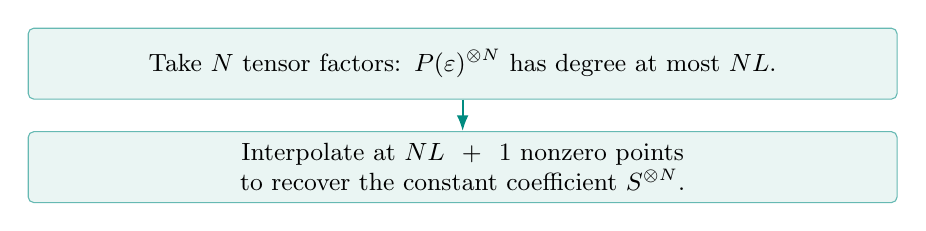
\begin{tikzpicture}[node distance=4mm]
    \node[flow,text width=10.8cm] (power)
      {Take $N$ tensor factors: $P(\varepsilon)^{\otimes N}$ has degree at most $NL$.};
    \node[flow,text width=10.8cm,below=of power] (eval)
      {Interpolate at $NL+1$ nonzero points to recover the constant coefficient $S^{\otimes N}$.};
    \draw[arrow] (power) -- (eval);
  \end{tikzpicture}
  \end{center}
  \[
    \rank(S^{\otimes N})\le(NL+1)\rank(T)^N.
  \]
  \takeaway{Take $N$-th roots: $(NL+1)^{1/N}\to1$. Thus
    $\displaystyle\widetilde R(S)\le\rank(T)$.}
  \source{Lemma 3.1 and Appendix D; standard interpolation conversion~\cite{interpolation}.
  Interpolation is an exact linear combination of evaluations. For matrix
  multiplication, a fixed tensor power supplies a block algorithm to recurse.}
\end{frame}

% Toolkit 12. Introduce characters before convolution values and their parameters.
\begin{frame}{Tensor characters turn constructions into inequalities}
  Rank and asymptotic rank are subadditive and submultiplicative.
  Our counting argument uses \textbf{exact addition and multiplication}.
  \par\medskip
  A \textbf{tensor character} $\lambda$ assigns nonnegative values with these rules:
  \par\medskip
  \begin{center}
    \renewcommand{\arraystretch}{1.5}
    \begin{tabular}{@{}ll@{}}
      Independent computations & $\lambda(S\oplus T)=\lambda(S)+\lambda(T)$\\
      Tensor products & $\lambda(S\otimes T)=\lambda(S)\lambda(T)$\\
      One scalar product & $\lambda(abc)=1$\\
      Restriction & $T\ge S\ \Longrightarrow\ \lambda(T)\ge\lambda(S)$
    \end{tabular}
  \end{center}
  \medskip
  \takeaway{Every character gives a lower bound on asymptotic rank:
    $\displaystyle\lambda(T)\le\widetilde R(T)$.}
  \source{Section 3; rank properties:~\cite[Section 4.1]{spectra}.
  The rules give $\lambda(T)^N=\lambda(T^{\otimes N})\le\rank(T^{\otimes N})$;
  take $N$-th roots and the limit.}
\end{frame}

% Toolkit 13. State spectral duality separately from the character lower bound.
\begin{frame}{Strassen's spectral theorem}
  For every nonzero tensor $T$ over $\CC$:
  \begin{block}{Spectral duality}
    \[
      \widetilde R(T)=\max_{\lambda}\lambda(T),
    \]
    where the maximum ranges over all tensor characters.
  \end{block}
  \medskip
  A bound $\lambda(T)\le R$ for \textbf{every} character implies
  $\widetilde R(T)\le R$.
  \par\medskip
  \takeaway{For $M=\cmm{q}{q}{q}$, with integer $q\ge2$,
    \[
      \lambda(M)\le R\ \text{for every }\lambda
        \quad\Longrightarrow\quad\omega\le\log_q R.
    \]}
  \source{Theorem 3.2 of the note; Strassen~\cite[Theorem 3.8]{strassen} and
  Wigderson--Zuiddam~\cite[Corollary 3.30, author version]{spectra}.
  The supremum is attained. The exponent implication uses the fixed-power
  block algorithm from slide 19.}
\end{frame}

\begin{frame}{Convolution and dot-product tensors}
  Write $x^{(X)}=x$, $x^{(Y)}=y$, $x^{(Z)}=z$ for the three groups of variables.
  \par\medskip
  \begin{columns}[T,onlytextwidth]
    \begin{column}{0.52\textwidth}
      \textbf{Convolution}
      \[
        C_{ij}(r,s)=\sum_{h=0}^{r-1}\sum_{\ell=0}^{s-1}
        x_h^{(i)}x_\ell^{(j)}x_{h+\ell}^{(k)}.
      \]
      Encodes polynomial multiplication. Inputs have $r,s$ coefficients;
      the output has $r+s-1$ coefficients.
    \end{column}
    \begin{column}{0.44\textwidth}
      \textbf{Oriented dot products}
      \[
      \begin{aligned}
        B_X(q)&=x\sum_{h=1}^{q}y_hz_h,\\
        B_Y(q)&=y\sum_{h=1}^{q}x_hz_h,\\
        B_Z(q)&=z\sum_{h=1}^{q}x_hy_h.
      \end{aligned}
      \]
    \end{column}
  \end{columns}
  \medskip
  \takeaway{$C_{ij}$: input legs $i,j$; output leg $k$.\newline
    $B_i$: leg $i$ is scalar; the other two legs each have $q$ coordinates.}
  \source{Definitions: Section 2 of the note; convolution background~\cite{convolution}.
  The legs $i,j,k$ are distinct elements of $\{X,Y,Z\}$;
  $r,s,q$ are positive integers.}
\end{frame}

\begin{frame}{Three parameters describe dot-product values}
  Fix an arbitrary tensor character $\lambda$.
  For the dot-product tensor $B_X(q)=x\sum_{j=1}^{q}y_jz_j$,
  and the other two orientations, pairing indices gives
  \[
    B_i(q)\otimes B_i(r)\cong B_i(qr).
  \]
  Character multiplicativity and monotonicity in $q$ force a power law.
  \par\medskip
  \takeaway{One exponent per orientation determines all dot-product values:
    \[
      \lambda(B_i(q))=q^{p_i},\qquad
      p_i\in[0,1],\quad i\in\{X,Y,Z\}.
    \]}
  \source{Section 3. The three parameters need not be equal.
  Interpolation also gives monotonicity under degeneration.
  Spectral duality~\cite{strassen,spectra} will turn character bounds into rank bounds.}
\end{frame}

% Derive the matrix-tensor factorization by tracking the three shared indices.
\begin{frame}{Matrix multiplication factors into three dot products}
  In each term $a_{ik}b_{kj}c_{ij}$, the $a,b,c$ variables belong to
  legs $X,Y,Z$, respectively.
  \begin{center}
    \renewcommand{\arraystretch}{1.15}
    \begin{tabular}{@{}lll@{}}
      \toprule
      Index & Appears in & Dot-product factor\\
      \midrule
      Row $i\in[A]$ & $a_{ik},c_{ij}$ & $B_Y(A)$\\
      Inner $k\in[B]$ & $a_{ik},b_{kj}$ & $B_Z(B)$\\
      Column $j\in[C]$ & $b_{kj},c_{ij}$ & $B_X(C)$\\
      \bottomrule
    \end{tabular}
  \end{center}
  The subscript names the \textbf{scalar leg}. Tensoring pairs the indices:
  \[
    \cmm{A}{B}{C}\cong B_Y(A)\otimes B_Z(B)\otimes B_X(C).
  \]
  \takeaway{$\displaystyle
    \lambda(\cmm{A}{B}{C})
      =\lambda(B_Y(A))\lambda(B_Z(B))\lambda(B_X(C))
      =A^{p_Y}B^{p_Z}C^{p_X}.
  $}
  \source{Sections 2--3. Pairing the factor coordinates gives precisely
  $a_{ik},b_{kj},c_{ij}$; coordinates on scalar legs have dimension one.
  The last line uses character multiplicativity and $\lambda(B_i(q))=q^{p_i}$.
  Dimensions $A,B,C$ are positive integers.}
\end{frame}

\begin{frame}{Shared sectors give a power-sum inequality}
  The pieces may share variables on leg $i$; their variables on the other
  two legs belong to disjoint, matched sectors.
  \medskip
  \begin{columns}[T,onlytextwidth]
    \begin{column}{0.43\textwidth}
      \textbf{Example: a shared first leg}
      \[
        T=\underbrace{xy_1z_1}_{T_1}
          +\underbrace{xy_2z_2}_{T_2}.
      \]
      This is $B_X(2)$, so
      \[
      \begin{gathered}
        \lambda(T)=2^{p_X},\\
        \lambda(T_1)=\lambda(T_2)=1.
      \end{gathered}
      \]
    \end{column}
    \begin{column}{0.53\textwidth}
      \begin{block}{The general rule, for $p_i>0$}
      If $T\degen\sum_h T_h$ has this sector structure,
      \[
        \lambda(T)^{1/p_i}
        \ge\sum_h\lambda(T_h)^{1/p_i}.
      \]
      \end{block}
      The next slides prove this using tensor powers, finite separation,
      and counting.
    \end{column}
  \end{columns}
  \source{Lemma 3.3. The common variable $x$ makes the example a shared-leg sum.
  The following slides prove the rule using finite separation and multinomial
  counting. The separation construction is in the holdout slides.}
\end{frame}

% Power-sum proof 1. Identify the words and retain one multiplicity group.
\begin{frame}{Tensor powers group sector choices by multiplicity}
  Suppose $T\degen\sum_{h=1}^{s}T_h$ has matched sectors sharing leg $i$.
  Fix a character $\lambda$ with $p=p_i>0$.
  \par\medskip
  Expanding $(\sum_h T_h)^{\otimes N}$ gives a sector for every word
  $w_1\cdots w_N\in\{1,\ldots,s\}^N$.
  For example, $112$ means $T_1\otimes T_1\otimes T_2$:
  \[
    \underbrace{112,\quad121,\quad211}_{\text{multiplicities }(n_1,n_2)=(2,1)}.
  \]
  Fixing counts $n_1+\cdots+n_s=N$ gives
  \[
    M=\binom{N}{n_1,\ldots,n_s},\qquad
    U=\bigotimes_{h=1}^{s}T_h^{\otimes n_h}.
  \]
  \takeaway{Retain these $M$ words by zeroing coordinates on the two
    unshared legs. Each word has the factors of $U$, in a different order.}
  \source{Section 3, proof of Lemma 3.3. Here $N\ge1$ and the $n_h\ge0$ are
  integers. Independent reordering of the words' factors becomes valid after
  applying the separation lemma.}
\end{frame}

% Power-sum proof 2. State the separation lemma before using it.
\begin{frame}[label=finite-separation-lemma]{Finite separation: give every sector its own variables}
  Let $Q=F_1+\cdots+F_M$, with $M\ge1$ sectors sharing leg $i$.
  Their variables on each of the other two legs are pairwise disjoint.
  \begin{block}{Finite-separation lemma}
    \[
      (2M)Q\degen
      \bigoplus_{w=1}^{M}\bigl(F_w\otimes B_i(M)\bigr).
    \]
  \end{block}
  Here $(2M)Q$ means \textbf{$2M$ independent copies} of $Q$.
  \par\medskip
  \begin{columns}[T,onlytextwidth]
    \begin{column}{0.46\textwidth}
      \centering\textbf{Before: one shared leg}\par\smallskip
      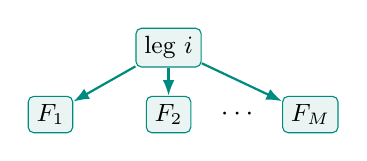
\begin{tikzpicture}[x=1cm,y=1cm,
        sector/.style={draw=teal,fill=pale,rounded corners=2pt,
          inner sep=3pt,font=\small}]
        \node[sector] (f1) at (0,0) {$F_1$};
        \node[sector] (f2) at (1.5,0) {$F_2$};
        \node at (2.4,0) {$\cdots$};
        \node[sector] (fm) at (3.3,0) {$F_M$};
        \node[sector] (shared) at (1.5,0.85) {leg $i$};
        \draw[arrow] (shared) -- (f1);
        \draw[arrow] (shared) -- (f2);
        \draw[arrow] (shared) -- (fm);
      \end{tikzpicture}
    \end{column}
    \begin{column}{0.52\textwidth}
      \centering\textbf{After: independent sectors}\par\smallskip
      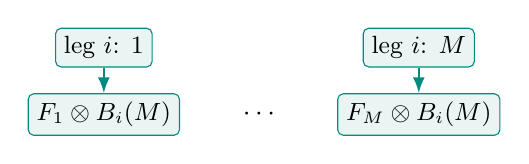
\begin{tikzpicture}[x=1cm,y=1cm,
        sector/.style={draw=teal,fill=pale,rounded corners=2pt,
          inner sep=3pt,font=\small}]
        \node[sector] (g1) at (0,0) {$F_1\otimes B_i(M)$};
        \node[sector] (gm) at (4,0) {$F_M\otimes B_i(M)$};
        \node at (2,0) {$\cdots$};
        \node[sector] (i1) at (0,0.85) {leg $i$: $1$};
        \node[sector] (im) at (4,0.85) {leg $i$: $M$};
        \draw[arrow] (i1) -- (g1);
        \draw[arrow] (im) -- (gm);
      \end{tikzpicture}
    \end{column}
  \end{columns}
  \source{Lemma 2.1(1); appendix ``Finite separation of a shared leg''.
  \hyperlink{finite-separation-setup}{Six holdout slides} give the construction:
  a root-of-unity filter of length $2M$, followed by $\varepsilon$-weights
  that retain matching sector labels.}
\end{frame}

% Power-sum proof 3. Apply the lemma, then reorder the retained words.
\begin{frame}{Finite separation makes the words independent}
  Let $Q=\sum_{w=1}^{M}F_w$ be the retained word sectors.
  The previous retention step gives $T^{\otimes N}\degen Q$;
  these sectors share leg $i$.
  \begin{block}{Apply the lemma, then reorder factors}
    \[
    \begin{aligned}
      (2M)T^{\otimes N}\degen(2M)Q
        &\degen\bigoplus_{w=1}^{M}\bigl(F_w\otimes B_i(M)\bigr)\\
        &\cong\bigoplus_{w=1}^{M}\bigl(U\otimes B_i(M)\bigr).
    \end{aligned}
    \]
  \end{block}
  \medskip
  \takeaway{All three legs now distinguish $w$, so each word's factors
    can be reordered independently to give $U$.}
  \source{First step: retain the multiplicity group in each copy.
  Second: the \hyperlink{finite-separation-lemma}{finite-separation lemma}
  (Lemma 2.1(1)), proved in \hyperlink{finite-separation-setup}{six holdout slides}.
  Third: all words have the same factor multiplicities, so $F_w\cong U$.}
\end{frame}

% Power-sum proof 4. Account for copies, tensor factors, and the dot-product value.
\begin{frame}{A multiplicity group gives one character inequality}
  Apply $\lambda$ to the separation degeneration, using monotonicity from
  interpolation. Since $p=p_i>0$, we have $\lambda(B_i(M))=M^p$:
  \[
    2M\,\lambda(T)^N\ge
      \underbrace{M}_{\text{copies}}\,
      \underbrace{\prod_h\lambda(T_h)^{n_h}}_{\lambda(U)}\,
      \underbrace{M^p}_{\lambda(B_i(M))}.
  \]
  Cancel $M$, take the power $1/p$, and set
  \[
    a_h=\lambda(T_h)^{1/p}.
  \]
  \takeaway{$\displaystyle
    M\prod_{h=1}^{s}a_h^{n_h}
      \le2^{1/p}\lambda(T)^{N/p}.
  $}
  \medskip
  The bound on the right is the same for every multiplicity tuple.
  \source{Lemma 3.3 and the appendix ``Counting and rescaling''.
  The calculation uses character additivity, multiplicativity, and
  monotonicity under degeneration; the latter follows from interpolation
  (Lemma 3.1; also shown in backup).}
\end{frame}

% Power-sum proof 5. Sum the type bounds, then remove the polynomial factor.
\begin{frame}{Sum over multiplicities, then take roots}
  There are at most $(N+1)^s$ tuples with $n_1+\cdots+n_s=N$.
  Sum their bounds and use the multinomial theorem:
  \[
  \begin{aligned}
    \left(\sum_{h=1}^{s}a_h\right)^N
      &=\sum_{\substack{n_1+\cdots+n_s=N\\n_h\ge0}}
        \binom{N}{n_1,\ldots,n_s}\prod_h a_h^{n_h}\\
      &\le(N+1)^s2^{1/p}\lambda(T)^{N/p}.
  \end{aligned}
  \]
  Take $N$-th roots and let $N\to\infty$:
  \[
    \sum_h a_h\le
      \underbrace{(N+1)^{s/N}2^{1/(pN)}}_{\longrightarrow\,1}
      \lambda(T)^{1/p}.
  \]
  \takeaway{This proves Lemma~3.3:\quad$\displaystyle
    \lambda(T)^{1/p_i}\ge\sum_h\lambda(T_h)^{1/p_i}.
  $}
  \source{Lemma 3.3 and the appendix ``Counting and rescaling''.
  The number of sectors $s$ and the character's parameter $p=p_i>0$
  stay fixed as $N\to\infty$.}
\end{frame}

% State the splittings here; all coordinate interpretations and proofs are in backup.
\begin{frame}[label=two-sector-splitting]{Two-sector splitting lemma}
  Fix integers $r\ge1$, $s\ge2$, and distinct legs $i,j$.
  \begin{block}{Two matched sectors}
    \[
      C_{ij}(r,s)\otimes B_i(2)\degen T_++T_-,
      \qquad T_\pm\cong C_{ij}(r,s\pm1).
    \]
    The sectors share leg $i$ and use disjoint coordinates on the other legs.
  \end{block}
  \source{Lemma 2.1(2); \cite[Lemma 4.1]{nine-fourths}.
  \hyperlink{two-sector-proof}{Coordinate interpretation and proof in backup.}}
\end{frame}

\begin{frame}[label=three-sector-splitting]{Three-sector splitting lemma}
  Fix integers $r,s\ge1$ and distinct legs $i,j,k$.
  \begin{block}{Three matched sectors}
    \[
    \begin{gathered}
      C_{ij}(r,3s+r-1)\degen T_1+T_2+T_3,\\
      T_1,T_2\cong C_{ij}(r,s),\qquad T_3\cong C_{ik}(r,s).
    \end{gathered}
    \]
    The sectors share leg $i$ and use pairwise disjoint coordinates
    on the other legs.
  \end{block}
  \source{Lemma 2.1(3); \cite[Lemma 4.2]{nine-fourths}.
  \hyperlink{three-sector-proof}{Coordinate interpretation and proof in backup.}}
\end{frame}

% Apply the shared-leg power-sum rule only after both splittings are explicit.
\begin{frame}{The splittings give two character inequalities}
  Fix a character $\lambda$, put $p=p_i>0$, and write
  $f_{ij}(r,s):=\lambda(C_{ij}(r,s))$.
  \begin{block}{Two sectors: neighboring lengths}
    Since $\lambda(B_i(2))=2^p$,
    \[
      2f_{ij}(r,s)^{1/p}
        \ge f_{ij}(r,s+1)^{1/p}+f_{ij}(r,s-1)^{1/p}.
    \]
    This is discrete concavity of $s\mapsto f_{ij}(r,s)^{1/p}$.
  \end{block}
  \begin{block}{Three sectors: coupled orientations}
    \[
      f_{ij}(r,3s+r-1)^{1/p}
        \ge2f_{ij}(r,s)^{1/p}+f_{ik}(r,s)^{1/p}.
    \]
    The same parameter $p_i$ controls both orientations, since leg $i$ is shared.
  \end{block}
  \source{Lemmas 2.1 and 3.3. Character multiplicativity evaluates the
  two-sector source; the power-sum rule evaluates the shared sectors.
  The first inequality requires $r\ge1,s\ge2$; the second $r,s\ge1$.}
\end{frame}

% Combine replication with its purpose; additional profile properties are in backup.
\begin{frame}{Replication lets us compare all scales}
  Replication into $m$ independent copies gives
  \[
    C_{ij}(mr,ms)\degen mC_{ij}(r,s)
    \quad\Longrightarrow\quad
    f_{ij}(mr,ms)\ge m f_{ij}(r,s).
  \]
  Normalize the lengths; the limit exists for $r,s>0$:
  \[
    g_{ij}(r,s)=\lim_{m\to\infty}
      \frac{f_{ij}(\lceil mr\rceil,\lceil ms\rceil)}{m}.
  \]
  For $p=p_i>0$, powered concavity ($0<\delta<s$) and tripling become
  \[
  \begin{aligned}
    2g_{ij}(r,s)^{1/p}
      &\ge g_{ij}(r,s-\delta)^{1/p}+g_{ij}(r,s+\delta)^{1/p},\\
    g_{ij}(r,3s+r)^{1/p}
      &\ge2g_{ij}(r,s)^{1/p}+g_{ik}(r,s)^{1/p}.
  \end{aligned}
  \]
  The additive $-1$ becomes $-1/m\to0$ after rescaling.
  \par\smallskip
  \takeaway{The profiles are continuous and homogeneous:
    $\displaystyle g_{ij}(tr,ts)=t\,g_{ij}(r,s)$.}
  \source{Lemmas 2.2 and 4.1; Appendices E--F. Polynomial division and evaluation
  give replication. Common-scale approximation preserves the inequalities;
  additional profile properties are in backup.}
\end{frame}

% State the two one-variable profiles and their inequalities before using slopes.
\begin{frame}{Concavity and tripling couple two profiles}
  Fix a leg $i$ with $p_i>0$; let $j,k$ be the other legs. Write
  \[
    P(s):=P_{ij}(s)=g_{ij}(1,s)^{1/p_i},\qquad
    Q(s):=P_{ik}(s)=g_{ik}(1,s)^{1/p_i}.
  \]
  Both profiles are positive and nondecreasing. Their inequalities are
  \par\medskip
  \begin{columns}[T,onlytextwidth]
    \begin{column}{0.48\textwidth}
      \textbf{Concavity}, $0<\delta<s$
      \[
      \begin{aligned}
        2P(s)&\ge P(s-\delta)+P(s+\delta),\\
        2Q(s)&\ge Q(s-\delta)+Q(s+\delta).
      \end{aligned}
      \]
    \end{column}
    \begin{column}{0.48\textwidth}
      \textbf{Tripling}, $s>0$
      \[
      \begin{aligned}
        P(3s+1)&\ge2P(s)+Q(s),\\
        Q(3s+1)&\ge2Q(s)+P(s).
      \end{aligned}
      \]
    \end{column}
  \end{columns}
  \medskip
  \takeaway{We will prove that $\displaystyle
    \lim_{s\to\infty}\frac{P(s)}s
    =\lim_{s\to\infty}\frac{Q(s)}s=L_i>0$.
  }
  \source{Rescaled-profile inequalities (Lemma 4.1), with $r=1$.
  The second tripling inequality exchanges $j$ and $k$; the parameter $p_i$
  stays the same.}
\end{frame}

% Concave secants have limits; the two tripling inequalities identify them.
\begin{frame}{Tripling forces the limiting slopes to agree}
  The secant slopes $(P(s)-P(1))/(s-1)$ are nonnegative and decrease
  with $s>1$. Thus their finite limit exists and equals
  \[
    L_P:=\lim_{s\to\infty}\frac{P(s)-P(1)}{s-1}
      =\lim_{s\to\infty}\frac{P(s)}s\ge0.
  \]
  Define $L_Q$ analogously for $Q$.
  \par\medskip
  Divide both tripling inequalities by $s$ and let $s\to\infty$.
  Since $P(3s+1)/s\to3L_P$, and likewise for $Q$,
  \[
  \begin{aligned}
    3L_P&\ge2L_P+L_Q &&\Longrightarrow\quad L_P\ge L_Q,\\
    3L_Q&\ge2L_Q+L_P &&\Longrightarrow\quad L_Q\ge L_P.
  \end{aligned}
  \]
  \takeaway{$L_P=L_Q=:L_i\ge0$. It remains to prove $L_i>0$.}
  \source{Proof of Lemma 5.1, Appendix G.
  Monotonicity makes the secants nonnegative; concavity makes them decrease.}
\end{frame}

% Iterate the coupled inequalities to exclude a zero common slope.
\begin{frame}{Iterated tripling makes the common slope positive}
  Put $R=P+Q>0$. Adding the tripling inequalities gives
  \[
    R(3s+1)\ge3R(s),\qquad
    \lim_{s\to\infty}\frac{R(s)}s=2L_i.
  \]
  Fix $s>0$. Iterate at
  \[
    s_0=s,\quad s_{n+1}=3s_n+1
    \quad\Longrightarrow\quad
    s_n=3^n\left(s+\tfrac12\right)-\tfrac12.
  \]
  Then $R(s_n)\ge3^nR(s)$.
  Since $R(s_n)/s_n\to2L_i$ and $s_n/3^n\to s+\tfrac12$,
  \[
    R(s)\le\lim_{n\to\infty}\frac{R(s_n)}{3^n}
      =2L_i\left(s+\tfrac12\right)=L_i(2s+1).
  \]
  \takeaway{$\displaystyle L_i\ge\frac{R(s)}{2s+1}>0$:
    the common slope is positive.}
  \source{Proof of Lemma 5.1, Appendix G.
  The same estimate $P(s)+Q(s)\le L_i(2s+1)$ will bound the offsets.}
\end{frame}

\begin{frame}{The two residuals share a budget of one}
  Divide $P(s)+Q(s)\le L_i(2s+1)$ by $L_i>0$ and subtract $2s$:
  \[
    \underbrace{\left(\frac{P(s)}{L_i}-s\right)}_{a(s)}
    +\underbrace{\left(\frac{Q(s)}{L_i}-s\right)}_{b(s)}\le1.
  \]
  \begin{columns}[c,onlytextwidth]
    \begin{column}{0.49\textwidth}
      Concavity makes $a,b$ nonnegative and nondecreasing.
      The budget bounds each by $1$, so both limits exist:
      \[
      \begin{aligned}
        c_{ij}&:=\lim_{s\to\infty}a(s),\\
        c_{ik}&:=\lim_{s\to\infty}b(s).
      \end{aligned}
      \]
    \end{column}
    \begin{column}{0.47\textwidth}
      \centering
      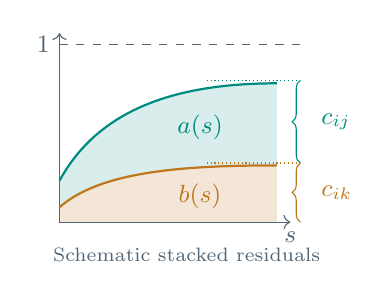
\begin{tikzpicture}[x=0.85cm,y=0.75cm,font=\small]
        \fill[amber!18] (0,0) -- (3.25,0) -- (3.25,.96)
          .. controls (1.8,.96) and (.6,.85) .. (0,.25) -- cycle;
        \fill[teal!15] (0,.25)
          .. controls (.6,.85) and (1.8,.96) .. (3.25,.96)
          -- (3.25,2.35)
          .. controls (1.8,2.35) and (.6,1.95) .. (0,.70) -- cycle;
        \draw[->,muted] (0,0) -- (3.45,0) node[below] {$s$};
        \draw[->,muted] (0,0) -- (0,3.2);
        \draw[dashed,muted] (0,3) node[left] {$1$} -- (3.7,3);
        \draw[thick,amber] (0,.25)
          .. controls (.6,.85) and (1.8,.96) .. (3.25,.96);
        \draw[thick,teal] (0,.70)
          .. controls (.6,1.95) and (1.8,2.35) .. (3.25,2.35);
        \draw[densely dotted,amber] (2.2,1) -- (3.55,1);
        \draw[densely dotted,teal] (2.2,2.4) -- (3.55,2.4);
        \node[amber] at (2.1,.44) {$b(s)$};
        \node[teal] at (2.1,1.6) {$a(s)$};
        \draw[decorate,decoration={brace,amplitude=3pt},amber]
          (3.6,0) -- (3.6,1) node[midway,right=4pt] {$c_{ik}$};
        \draw[decorate,decoration={brace,amplitude=3pt},teal]
          (3.6,1) -- (3.6,2.4) node[midway,right=4pt] {$c_{ij}$};
        \node[muted,font=\scriptsize] at (1.9,-.55) {Schematic stacked residuals};
      \end{tikzpicture}
    \end{column}
  \end{columns}
  \takeaway{$c_{ij},c_{ik}\ge0$,\quad $c_{ij}+c_{ik}\le1$.\newline
    $L_i s\le P(s)\le L_i(s+c_{ij})$,\quad
    $L_i s\le Q(s)\le L_i(s+c_{ik})$.}
  \source{Lemma 5.1, Appendix G. The limits exist because the residuals
  are nondecreasing and bounded; $a(s)\le c_{ij}$ and $b(s)\le c_{ik}$.}
\end{frame}

% Finite increments give relative growth without differentiating the profiles.
\begin{frame}{Finite increments give relative growth}
  Assume $p_i>0$. The common-slope lemma gives, for $s,t>0$,
  \[
    P_{ij}(s+t)\ge P_{ij}(s)+L_it,\qquad
    P_{ij}(s)\le L_i(s+c_{ij}).
  \]
  Divide the first inequality by $P_{ij}(s)>0$ and use the second:
  \[
    \frac{P_{ij}(s+t)}{P_{ij}(s)}
    \ge1+\frac{L_it}{P_{ij}(s)}
    \ge1+\frac{t}{s+c_{ij}}.
  \]
  Since $g_{ij}(r,s)=rP_{ij}(s/r)^{p_i}$, homogeneity gives
  \takeaway{$\displaystyle
    \frac{g_{ij}(r,s+t)}{g_{ij}(r,s)}
    \ge\left(1+\frac{t}{s+c_{ij}r}\right)^{p_i}
    \qquad(r,s,t>0).
  $}
  \source{Lemma 5.1 and Proposition 5.2.
  The lower bound applies to every positive finite increment.}
\end{frame}

\begin{frame}{Homogeneity gives the pair inequality}
  Assume $p_i,p_j>0$. Increase $r$ by $\varepsilon r$, then $s$ by
  $\varepsilon s$. Input interchange gives the first increment bound:
  \[
  \begin{aligned}
    1+\varepsilon
    &=\frac{g_{ij}((1+\varepsilon)r,(1+\varepsilon)s)}{g_{ij}(r,s)}\\
    &\ge
    \left(1+\frac{\varepsilon r}{r+c_{ji}s}\right)^{p_j}
    \left(1+\frac{\varepsilon s}{s+c_{ij}(1+\varepsilon)r}\right)^{p_i}.
  \end{aligned}
  \]
  Take logarithms, divide by $\varepsilon$, and let $\varepsilon\downarrow0$:
  \takeaway{$\displaystyle
    \frac{p_is}{s+c_{ij}r}+\frac{p_jr}{r+c_{ji}s}\le1
    \qquad(r,s>0).
  $}
  \source{Proposition 5.2. The only limit used is
  $\log(1+\varepsilon x)/\varepsilon\to x$.
  For $p_i=0$, set its two offsets to zero; pairs involving it satisfy the
  bound directly because the remaining summand is at most $p_j\le1$.}
\end{frame}

% Choose the three length ratios to match the desired objective.
\begin{frame}{The weighted reciprocal bound}
  For any positive weights $w_1,w_2,w_3$, our target is
  \takeaway{$\displaystyle
    \sum_iw_ip_i\le
    \frac14\left(\sum_i\frac1{w_i}\right)
             \left(\sum_{i<j}w_iw_j\right).
  $}
  \medskip
  For each unordered pair $\{i,j\}$, set $r=1/w_i$, $s=1/w_j$
  in the pair inequality and multiply by $w_iw_j$:
  \[
    w_iw_j\ge
    \frac{p_iw_i^2}{w_i/w_j+c_{ij}}
    +\frac{p_jw_j^2}{w_j/w_i+c_{ji}}.
  \]
  We will sum the three inequalities and use $c_{ij}+c_{ik}\le1$.
  \source{Proposition 5.3. The offsets are fixed independently of the
  chosen lengths and weights. No equality among the parameters is assumed.}
\end{frame}

\begin{frame}{The reciprocal inequality eliminates the offsets}
  Summing over the three unordered pairs and grouping by $p_i$ gives
  \[
    \sum_{i<j}w_iw_j\ge
    \sum_i p_iw_i^2\left(
      \frac1{w_i/w_j+c_{ij}}+\frac1{w_i/w_k+c_{ik}}\right).
  \]
  Here $j,k$ are the other indices in the summand indexed by $i$.
  For positive $x,y$,
  \[
    \frac1x+\frac1y\ge\frac4{x+y}.
  \]
  Apply this and $c_{ij}+c_{ik}\le1$:
  \[
    \sum_{i<j}w_iw_j
    \ge4\sum_i\frac{p_iw_i^2}{w_i/w_j+w_i/w_k+1}
    =\frac{4\sum_iw_ip_i}{\sum_{\ell=1}^3 1/w_\ell}.
  \]
  This proves the weighted bound.
  \source{Proposition 5.3. All denominators are positive, and $p_i\ge0$
  preserves each lower bound.}
\end{frame}

\begin{frame}{Character bounds give arithmetic algorithms}
  \textbf{Published spectral input:}
  \[
    \widetilde R(T)=\max_{\lambda}\lambda(T),\qquad
    \widetilde R(T)=\inf_{N\ge1}\rank(T^{\otimes N})^{1/N}.
  \]
  If every character has $a p_Y+b p_Z+c p_X\le E$:
  \begin{enumerate}
    \item Choose a fixed large base $B$ and round the block dimensions upward.
    \item Spectral duality supplies a finite exact rank identity for a tensor power.
    \item Apply that identity recursively to matrix blocks; pad to the input size.
  \end{enumerate}
  \medskip
  \takeaway{For every positive exponent slack, we obtain a fixed finite
  block algorithm. Recursion gives the claimed arithmetic exponent.}
  \source{Theorem 3.2~\cite{strassen,spectra} and Lemma 6.1.
  Linear combinations cost $O(\ell R^\ell)$ over $\ell$ recursion levels.
  The exponent statement does not provide a practical small-base implementation.}
\end{frame}

\begin{frame}{Substitute the shape into the weighted bound}
  For $a,b,c>0$, take $w=(a,b,c)$ and
  $(p_1,p_2,p_3)=(p_Y,p_Z,p_X)$. For every character,
  \[
  \begin{aligned}
    ap_1+bp_2+cp_3
    &\le\frac14\left(\frac1a+\frac1b+\frac1c\right)(ab+ac+bc)\\[3pt]
    &=\frac{a+b+c}{2}
      +\frac14\left(\frac{ab}{c}+\frac{ac}{b}+\frac{bc}{a}\right).
  \end{aligned}
  \]
  The character-to-algorithm implication now gives
  \takeaway{$\displaystyle
    \omega(a,b,c)\le\frac{a+b+c}{2}
      +\frac14\left(\frac{ab}{c}+\frac{ac}{b}+\frac{bc}{a}\right).
  $}
  \source{Proposition 5.3 and Lemma 6.1.
  Zero character parameters were included in the pair inequality;
  this bound holds for every positive shape, including the thin threshold.}
\end{frame}

\begin{frame}{The thin case follows by padding}
  Assume $a\ge b>0$ and put
  \[
    c_0=\frac{ab}{a+b}.
  \]
  Padding makes $\omega$ nondecreasing in each argument.
  For $0\le c\le c_0$,
  \takeaway{$\displaystyle
    \omega(a,b,c)
    \le\omega(a,b,c_0)
    \le a+b.
  $}
  \source{Proof of Theorem 1.1. The bound on the preceding slide applies
  at $c_0>0$. The matching size lower bound gives
  $\omega(a,b,c)=a+b$ throughout the thin range.}
\end{frame}

\begin{frame}{Applications through established tradeoffs}
  \begin{center}
  \renewcommand{\arraystretch}{1.25}
  \begin{tabular}{@{}p{7.8cm}l@{}}
  \toprule
  Problem & Running time\\
  \midrule
  Directed unweighted APSP: Zwick's balance~\cite{zwick} & $O(n^{2.5})$\\
  Combining with Alman--Vassilevska Williams~\cite{aw} & $O(n^{2.4999})$\\
  One LCA per pair in a DAG~\cite{lca} & $O(n^{(3+\sqrt3)/2})$\\
  Exact all-pairs Hamming distance~\cite{hamming,dominance} & $O(n^{(13-\sqrt7)/4})$\\
  Minimum / maximum Boolean witnesses~\cite{witnesses} & $O(n^{2.5})$\\
  Sparse multiplication, $m\le n^{1.25}$~\cite{sparse} & $O(n^2)$\\
  \bottomrule
  \end{tabular}
  \end{center}
  \source{Section 7. The LCA and Hamming exponents are approximately
  $2.36603$ and $2.58856$, respectively.
  Hamming inputs are $n$ vectors of length $n$ over an unrestricted alphabet;
  sparse inputs have at most $m$ nonzeros each.}
\end{frame}

\begin{frame}{What the rectangular extension contributes}
  \begin{columns}[T,onlytextwidth]
    \begin{column}{0.48\textwidth}
      \textbf{Starting constructions}\par\medskip
      The two polynomial splittings recap~\cite{nine-fourths}.
      Finite separation adapts its shared-leg construction.\par\medskip
      \textbf{Standard tools}\par\medskip
      Multinomial counting, spectral duality, interpolation,
      the reciprocal inequality, and padding.
    \end{column}
    \begin{column}{0.48\textwidth}
      \textbf{Rectangular analysis}\par\medskip
      Keep all orientations; replicate and rescale convolution profiles;
      couple six offsets; sum the pair inequalities at reciprocal lengths.\par\medskip
      \textbf{Lean correspondence}\par\medskip
      The main bounds are checked with the published spectral theorem
      supplied explicitly as a hypothesis.
    \end{column}
  \end{columns}
  \vspace{3mm}
  \takeaway{$\displaystyle c\le\frac{ab}{a+b}\ \Longrightarrow\
  \omega(a,b,c)=a+b\qquad(a\ge b\ge c\ge0)$.}
  \source{The note makes no priority claim for standard tools or finite construction variants.
  Lean checks mathematical statements; some finite proof routes differ from the manuscript.
  The application algorithms are outside the formalization.}
\end{frame}

\renewcommand{\appendixname}{Backup}
\appendix

\begin{frame}[label=degeneration-rank-proof]{Backup: the degeneration target has rank three}
  The coefficients of $c_0$ and $c_1$ in
  $S=a_0b_0c_0+(a_0b_1+a_1b_0)c_1$ are the two matrices
  \[
    A=\begin{pmatrix}1&0\\0&0\end{pmatrix},\qquad
    B=\begin{pmatrix}0&1\\1&0\end{pmatrix}.
  \]
  A rank-two decomposition of $S$ would put both $A$ and $B$ in the span
  of two rank-one matrices. Since $A,B$ are independent, those matrices
  would have to span exactly the same plane.
  \[
    \alpha A+\beta B=\begin{pmatrix}\alpha&\beta\\\beta&0\end{pmatrix},
    \qquad \det(\alpha A+\beta B)=-\beta^2.
  \]
  Every nonzero rank-one matrix in this plane is therefore a multiple of $A$.
  Two independent rank-one generators cannot exist.
  \par\medskip
  \takeaway{Thus $\rank(S)>2$. Its three displayed monomials give
    $\rank(S)\le3$, so $\rank(S)=3$.}
  \source{Elementary slice-space proof over $\CC$; the same rank statement is in
  \cite[proof of Proposition 13, p.~131]{interpolation}.
  In a rank-two decomposition, the two bilinear factors are rank-one matrices;
  both output coefficients are linear combinations of them.
  \hyperlink{degeneration-example}{Return to the example.}}
\end{frame}

% Separation proof 1. Set up the coefficients and state the desired target.
\begin{frame}[label=finite-separation-setup]{Separation proof: start with a shared first leg}
  Work over $\CC$. Assume leg $X$ is shared, and write
  \[
    Q=\sum_{h=1}^{M}F_h,\qquad
    F_h=\sum_{a,b,c}\mu_{habc}\,x_a y_{h,b}z_{h,c}.
  \]
  The $x_a$ may be shared across sectors. The $y_{h,b}$ and $z_{h,c}$
  are already private to sector $h$.
  \begin{block}{The target has independent variables on every leg}
    \[
      S:=\bigoplus_{h=1}^{M}\bigl(F_h\otimes B_X(M)\bigr).
    \]
  \end{block}
  We construct an exact restriction, then a degeneration:
  \[
    (2M)Q\ \ge\ R\ \degen\ S.
  \]
  \source{Proof of Lemma 2.1(1), appendix ``Finite separation of a shared leg''.
  Here $M\ge1$; all coordinate sets are finite. Other shared-leg orientations
  follow by permuting the three legs.}
\end{frame}

% Separation proof 2. Give the three linear substitutions in each source copy.
\begin{frame}{Mix $2M$ copies using roots of unity}
  Set $L=2M$, and choose a primitive $L$-th root of unity $\zeta$.
  Label the independent copies by $\ell=0,\ldots,L-1$.
  \par\medskip
  In copy $\ell$, make these linear substitutions:
  \[
  \begin{aligned}
    x_a^{(\ell)}
      &\longmapsto\sum_{g=1}^{M}\zeta^{\ell g}X_{a,g},\\
    y_{h,b}^{(\ell)}
      &\longmapsto\sum_{u=1}^{M}\zeta^{\ell(u-h)}Y_{h,b,u},\\
    z_{h,c}^{(\ell)}
      &\longmapsto\frac1L\sum_{v=1}^{M}\zeta^{-\ell v}Z_{h,c,v}.
  \end{aligned}
  \]
  \takeaway{The new indices $g,u,v$ each run from $1$ to $M$.
    Each substitution acts on just one leg.}
  \source{All new coordinates are independent within each leg.
  The first-leg label is $g$; $u,v$ label coordinates on the other legs.
  Summing copies cancels unwanted combinations of these labels.}
\end{frame}

% Separation proof 3. Expand the substitutions and evaluate the finite filter.
\begin{frame}{The finite sum keeps exactly $g+u=h+v$}
  After summing the copies, the coefficient of
  $X_{a,g}Y_{h,b,u}Z_{h,c,v}$ is $\mu_{habc}$ times
  \[
    \frac1L\sum_{\ell=0}^{L-1}\zeta^{\ell(g+u-h-v)}
      =\begin{cases}
        1,&g+u-h-v\equiv0\pmod L,\\
        0,&\text{otherwise}.
      \end{cases}
  \]
  Since $|g+u-h-v|\le2M-2<L$, the only multiple of $L$ in this range is zero.
  Thus the filter keeps precisely $g+u=h+v$.
  \begin{block}{The exact restriction obtained so far}
    \[
      (2M)Q\ge R:=
      \sum_{\substack{h,g,u,v\\g+u=h+v}}\sum_{a,b,c}
      \mu_{habc}X_{a,g}Y_{h,b,u}Z_{h,c,v}.
    \]
  \end{block}
  \source{The filter identity is a finite geometric sum: if
  $\zeta^d\ne1$, then $\sum_{\ell=0}^{L-1}(\zeta^d)^\ell=0$;
  otherwise the sum is $L$. All $h,g,u,v$ lie in $\{1,\ldots,M\}$.}
\end{frame}

% Separation proof 4. Show that coordinate weights add to a nonnegative square.
\begin{frame}{Choose weights whose sum is a square}
  Every monomial of $R$ satisfies $g+u=h+v$.
  For $\varepsilon\ne0$, scale its coordinates by
  \[
  \begin{aligned}
    X_{a,g}&\longmapsto\varepsilon^{g^2}X_{a,g},\\
    Y_{h,b,u}&\longmapsto\varepsilon^{\,2hu-h^2}Y_{h,b,u},\\
    Z_{h,c,v}&\longmapsto\varepsilon^{-2hv}Z_{h,c,v}.
  \end{aligned}
  \]
  A surviving monomial acquires the total exponent
  \[
  \begin{aligned}
    g^2+2hu-h^2-2hv
      &=g^2+2h(u-v)-h^2\\
      &=g^2+2h(h-g)-h^2=(g-h)^2\ge0.
  \end{aligned}
  \]
  \takeaway{The exponent is zero exactly when $g=h$;
    all other retained monomials have positive exponent.}
  \source{Each weight depends only on indices of the coordinate being scaled,
  so the three substitutions act independently on the legs.
  The relation $u-v=h-g$ comes from the preceding filter.}
\end{frame}

% Separation proof 5. Take a coefficientwise limit, justifying singular weights.
\begin{frame}{Take the limit: matching labels survive}
  After scaling, the resulting tensor is
  \[
    P(\varepsilon)=
      \sum_{\substack{h,g,u,v\\g+u=h+v}}\sum_{a,b,c}
      \mu_{habc}\,\varepsilon^{(g-h)^2}
      X_{a,g}Y_{h,b,u}Z_{h,c,v}.
  \]
  \par\medskip
  As $\varepsilon\to0$, only $g=h$ survives. The filter equation then forces $u=v$:
  \[
    \lim_{\varepsilon\to0}P(\varepsilon)
      =\sum_{h=1}^{M}\sum_{a,b,c}\sum_{u=1}^{M}
        \mu_{habc}X_{a,h}Y_{h,b,u}Z_{h,c,u}
      =:S.
  \]
  \takeaway{For $\varepsilon\ne0$, $R\ge P(\varepsilon)$.
    The coefficientwise limit proves $R\degen S$, hence $(2M)Q\degen S$.}
  \source{Negative powers are allowed in the substitutions for nonzero
  $\varepsilon$. After the finite filter, every nonzero coefficient has
  the nonnegative exponent $(g-h)^2$, so the limit exists.}
\end{frame}

% Separation proof 6. Identify the dot-product factors and the direct sum.
\begin{frame}{Identify the independent sectors and dot products}
  Write $S=\sum_{h=1}^{M}S_h$, where
  \[
    S_h=\sum_{a,b,c}\sum_{u=1}^{M}
      \mu_{habc}X_{a,h}Y_{h,b,u}Z_{h,c,u}.
  \]
  Recall $B_X(M)=s\sum_{u=1}^{M}t_uw_u$.
  For each fixed $h$, pair the coordinates in $F_h\otimes B_X(M)$:
  {\centering
    \renewcommand{\arraystretch}{1.15}
    \begin{tabular}{@{}ccc@{}}
      \toprule
      $F_h$ coordinate & $B_X(M)$ coordinate & Paired coordinate\\
      \midrule
      $x_a$ & $s$ & $X_{a,h}$\\
      $y_{h,b}$ & $t_u$ & $Y_{h,b,u}$\\
      $z_{h,c}$ & $w_u$ & $Z_{h,c,u}$\\
      \bottomrule
    \end{tabular}
    \par}
  Thus $S_h\cong F_h\otimes B_X(M)$.
  All three legs carry $h$, so different $S_h$ use disjoint variables.
  \par\smallskip
  \takeaway{$\displaystyle
    (2M)Q\degen S\cong
      \bigoplus\nolimits_{h=1}^{M}\bigl(F_h\otimes B_X(M)\bigr).
  $}
  \source{This completes the proof of Lemma 2.1(1).
  Permuting the legs gives the same construction for any shared leg $i$.}
\end{frame}

% Two-sector proof setup: input/output semantics belong with the construction.
\begin{frame}[label=two-sector-proof]{Two-sector proof: the source and target maps}
  Fix $r\ge1,s\ge2$. Let $\mathcal P_d=\{p(t):\deg p<d\}$
  and $f\in\mathcal P_r$.
  \par\smallskip
  \begin{columns}[T,onlytextwidth]
    \begin{column}{0.47\textwidth}
      \textbf{Source: lengths $s,s$}
      \[
      \begin{gathered}
        (f,(a,b))\longmapsto(fa,fb),\\
        (a,b)\in\mathcal P_s\oplus\mathcal P_s.
      \end{gathered}
      \]
    \end{column}
    \begin{column}{0.49\textwidth}
      \textbf{Target: lengths $s+1,s-1$}
      \[
      \begin{gathered}
        (f,(p,h))\longmapsto(fp,fh),\\
        (p,h)\in\mathcal P_{s+1}\oplus\mathcal P_{s-1}.
      \end{gathered}
      \]
    \end{column}
  \end{columns}
  \takeaway{The first input $f$ is shared. The second input contains two
    independent polynomials; the two output blocks are disjoint.}
  \source{Lemma 2.1(2), appendix ``Splitting two polynomial products''.
  \hyperlink{two-sector-splitting}{Return to the lemma statement.}}
\end{frame}

% Tensor-product interpretation used by the two-sector construction.
\begin{frame}{Why tensoring with $B_X(2)$ gives two products}
  \textbf{Recall:} $B_X(2)=(uv_0)w_0+(uv_1)w_1$ encodes outputs $(uv_0,uv_1)$.
  \par\smallskip
  Read $X,Y$ as inputs and $Z$ as output. Both factors are bilinear maps:
  \[
  \begin{aligned}
    C_{XY}(r,s):\;&\mathcal P_r\times\mathcal P_s\to\mathcal P_{r+s-1},
      & (f,g)&\longmapsto fg,\\
    B_X(2):\;&\CC\times\CC^2\to\CC^2,
      & (u,(v_0,v_1))&\longmapsto(uv_0,uv_1).
  \end{aligned}
  \]
  The tensor product pairs corresponding input and output spaces:
  \[
    \underbrace{(\mathcal P_r\otimes\CC)}_{\mathcal P_r}
    \times
    \underbrace{(\mathcal P_s\otimes\CC^2)}_{\mathcal P_s\oplus\mathcal P_s}
    \ \longrightarrow
    \underbrace{(\mathcal P_{r+s-1}\otimes\CC^2)}_
      {\mathcal P_{r+s-1}\oplus\mathcal P_{r+s-1}}.
  \]
  For the standard basis $e_0,e_1$ of $\CC^2$, this map sends
  \[
    (f\otimes1,\ a\otimes e_0+b\otimes e_1)
      \longmapsto fa\otimes e_0+fb\otimes e_1.
  \]
  \takeaway{Thus $(f,(a,b))\mapsto(fa,fb)$: two products sharing $f$.}
  \source{The parameters $r,s,2$ specify dimensions, not function arguments.}
\end{frame}

% Two-sector proof 1. Give linear input maps for every r>=1 and s>=2.
\begin{frame}{Two-sector proof: encode the inputs}
  Fix arbitrary $r\ge1,s\ge2$. The inputs are
  $f\in\mathcal P_r$ and $(p,h)\in\mathcal P_{s+1}\oplus\mathcal P_{s-1}$.
  Keep $f$ unchanged.
  \par\medskip
  Write $p_s=[t^s]p$. For $\varepsilon\ne0$, encode the second input by
  \[
    E_\varepsilon:(p,h)\longmapsto(a,b),\qquad
    \begin{cases}
      a=p-p_s t^s-\varepsilon^{-1}th,\\
      b=\varepsilon^{-1}h+p_s t^{s-1}.
    \end{cases}
  \]
  Both have degree at most $s-1$: the leading term of $p$ was removed,
  and $\deg(th)\le s-1$.
  \par\medskip
  Apply the source bilinear map:
  \[
    (f,(p,h))\xrightarrow{\mathrm{id}\times E_\varepsilon}
    (f,(a,b))\longmapsto(U,V)=(fa,fb).
  \]
  \source{Lemma 2.1(2), appendix ``Splitting two polynomial products''.
  $E_\varepsilon$ is a linear map from $\mathcal P_{s+1}\oplus\mathcal P_{s-1}$
  to $\mathcal P_s\oplus\mathcal P_s$, independently of $f$.
  The definitions give $a+tb=p$.}
\end{frame}

% Two-sector proof 2. Give linear output maps and compute the needed coefficient.
\begin{frame}{Two-sector proof: decode the outputs}
  Put $m=r+s-2$, so $\deg U,\deg V\le m$. Decode the output pair linearly:
  \[
    D_\varepsilon:(U,V)\longmapsto(P,H_\varepsilon),\qquad
    \begin{cases}
      P=U+tV,\\
      H_\varepsilon=\varepsilon\bigl(V-[t^m]V\,t^m\bigr).
    \end{cases}
  \]
  The output lengths are $m+2=r+s$ for $P$ and $m=r+s-2$ for $H_\varepsilon$.
  \par\medskip
  Since $a+tb=p$,
  \[
    P=U+tV=f(a+tb)=fp.
  \]
  Expand the other product:
  \[
    V=\varepsilon^{-1}fh+p_s t^{s-1}f.
  \]
  Because $\deg(fh)\le r+s-3=m-1$, its top coefficient is
  \[
    [t^m]V=p_s f_{r-1},\qquad f_{r-1}=[t^{r-1}]f.
  \]
  \source{Coefficient extraction, deleting a coefficient, and shifting
  polynomial coefficients are linear output operations.
  The identity $[t^m]V=p_s f_{r-1}$ is used to analyze that output map.}
\end{frame}

% Two-sector proof 3. Compute the full error and identify the limit tensor.
\begin{frame}{Two-sector proof: the error vanishes}
  Substitute the expression for $V$ and its top coefficient:
  \[
  \begin{aligned}
    H_\varepsilon
      &=\varepsilon\bigl(V-p_s f_{r-1}t^{r+s-2}\bigr)\\
      &=fh+\varepsilon p_s t^{s-1}
        \bigl(f-f_{r-1}t^{r-1}\bigr)
        \xrightarrow{\varepsilon\to0}fh.
  \end{aligned}
  \]
  Encoding the second input, applying the source map, and decoding gives
  \[
    (f,(p,h))\longmapsto
    \bigl(fp,\ fh+\varepsilon p_s t^{s-1}
      (f-f_{r-1}t^{r-1})\bigr).
  \]
  The coefficients converge to those of $(fp,fh)$.
  The independent inputs $p,h$ have lengths $s+1,s-1$, and the two output
  blocks are disjoint; both products share $f$.
  \par\medskip
  \takeaway{$\displaystyle
    C_{XY}(r,s)\otimes B_X(2)\degen T_++T_-,
    \qquad T_\pm\cong C_{XY}(r,s\pm1).
  $}
  \source{This proves Lemma 2.1(2) for arbitrary $r\ge1,s\ge2$.
  If $r=1$, the error is identically zero. Permuting the legs gives
  every orientation $i,j$.}
\end{frame}

% Three-sector proof setup: identify the polynomial spaces and sector orientations.
\begin{frame}[label=three-sector-proof]{Three-sector proof: inputs and outputs}
  Fix $r,s\ge1$ and use $i=X,j=Y,k=Z$.
  Write $\mathcal P_d=\{p(t):\deg p<d\}$.
  \par\smallskip
  The source map is $(f,g)\mapsto fg$, with
  $f\in\mathcal P_r$ and $g\in\mathcal P_{3s+r-1}$.
  \par\smallskip
  The sectors share $f$; their $Y,Z$ coordinate blocks are disjoint:
  \begin{center}
    \renewcommand{\arraystretch}{1.2}
    \begin{tabular}{@{}lll@{}}
      \toprule
      Sector & Leg $j$ & Leg $k$\\
      \midrule
      $T_1,T_2$ & Input: $s$ coordinates & Output: $r+s-1$ coordinates\\
      $T_3$ & Output: $r+s-1$ coordinates & Input: $s$ coordinates\\
      \bottomrule
    \end{tabular}
  \end{center}
  \source{Lemma 2.1(3), appendix ``The three-sector splitting''.
  The middle sector's first-leg reversal identifies that individual tensor.
  \hyperlink{three-sector-splitting}{Return to the lemma statement.}}
\end{frame}

% Read the three-sector target using a fixed choice of output leg.
\begin{frame}{Three sectors, with $X,Y$ kept as the input legs}
  Split the second input into independent coefficient blocks:
  \[
    g=g_L+t^s q+t^{2s+r-1}g_R,\qquad
    g_L,g_R\in\mathcal P_s,\quad q\in\mathcal P_{r+s-1}.
  \]
  The target of the degeneration is the bilinear map
  \[
    (f,(g_L,q,g_R))\longmapsto
      \underbrace{\bigl(fg_L,\ M_f(q),\ fg_R\bigr)}_{\text{three output blocks}},
      \qquad f\in\mathcal P_r,
  \]
  where the middle output keeps $s$ coefficients of $fq$:
  \[
    M_f(q):=\sum_{v=0}^{s-1}[t^{r-1+v}](fq)\,t^v
      \in\mathcal P_s.
  \]
  The outer outputs $fg_L,fg_R$ each lie in $\mathcal P_{r+s-1}$.
  \par\medskip
  \takeaway{There are two input groups: $f$ and $(g_L,q,g_R)$.
    The name $C_{XZ}$ for the middle sector reads $Z$ as input and $Y$
    as output; the proof below makes this identification explicit.}
  \source{Here $[t^k]$ extracts the coefficient of $t^k$.
  The same three-leg tensor can be read with different choices of output leg.}
\end{frame}

% Three-sector proof 1. Partition all coordinates and define the substitutions.
\begin{frame}{Three-sector proof: partition the coordinates}
  Let $x_a,y_b$ be coefficients of $f,g$, and $z_c$ output labels.
  Set $n=3s+r-1$:
  \[
    C_{XY}(r,n)=\sum_{a=0}^{r-1}\sum_{b=0}^{n-1}x_a y_b z_{a+b}.
  \]
  Partition the integer indices of $Y$ and $Z$ into these disjoint intervals:
  \begin{center}
    \renewcommand{\arraystretch}{1.2}
    \begin{tabular}{@{}c|ccc@{}}
       & Left & Middle & Right\\
      \hline
      $Y$ & $[0,s-1]$ & $[s,2s+r-2]$ & $[2s+r-1,n-1]$\\
      $Z$ & $[0,s+r-2]$ & $[s+r-1,2s+r-2]$ & $[2s+r-1,n+r-2]$
    \end{tabular}
  \end{center}
  Encode the second input as
  $g_\varepsilon=g_L+\varepsilon t^s q+t^{2s+r-1}g_R$.
  Decode by dividing the middle output block by $\varepsilon$;
  leave the outer output blocks unchanged.
  \par\smallskip
  \takeaway{These are diagonal linear maps on the second input and the
    output. The first input $f$ is unchanged.}
  \source{Lemma 2.1(3), appendix ``The three-sector splitting''.
  All intervals include both endpoints; the $Y$ range is $0,\ldots,n-1$
  and the $Z$ range is $0,\ldots,n+r-2$.}
\end{frame}

% Three-sector proof 2. Prove the zero pattern and all epsilon exponents.
\begin{frame}{Three-sector proof: only matched blocks survive}
  A nonzero term has $c=a+b$ with $0\le a\le r-1$.
  \[
  \begin{aligned}
    b\le s-1&\ \Longrightarrow\ c\le s+r-2
      &&\text{(left $Y$ implies left $Z$)},\\
    b\ge2s+r-1&\ \Longrightarrow\ c\ge2s+r-1
      &&\text{(right $Y$ implies right $Z$)}.
  \end{aligned}
  \]
  The multipliers on the possible blocks are therefore
  \begin{center}
    \renewcommand{\arraystretch}{1.2}
    \begin{tabular}{@{}c|ccc@{}}
      $Y\backslash Z$ & Left & Middle & Right\\
      \hline
      Left & $1$ & $0$ & $0$\\
      Middle & $\varepsilon$ & $1$ & $\varepsilon$\\
      Right & $0$ & $0$ & $1$
    \end{tabular}
  \end{center}
  No supported term has a negative power of $\varepsilon$.
  As $\varepsilon\to0$, only the three matched blocks remain.
  \par\smallskip
  \takeaway{$C_{XY}(r,n)\degen T_1+T_2+T_3$, where $T_1,T_2$ are the
    left and right matched blocks, and $T_3$ is the middle matched block.}
  \source{Zero means no supported terms. An $\varepsilon$-block vanishes
  (and may be empty); the middle--middle factor is
  $\varepsilon\varepsilon^{-1}=1$.}
\end{frame}

% Three-sector proof 3. Identify both outer blocks by explicit translations.
\begin{frame}{Three-sector proof: identify the outer blocks}
  The left block has $0\le b<s$. Every $a+b$ lies in the left $Z$ interval, so
  \[
    T_1=\sum_{a=0}^{r-1}\sum_{v=0}^{s-1}x_a y_v z_{a+v}
      =C_{XY}(r,s).
  \]
  Put $A=2s+r-1$. In the right block, write $b=A+v$, with $0\le v<s$:
  \[
    T_2=\sum_{a=0}^{r-1}\sum_{v=0}^{s-1}
      x_a y_{A+v}z_{A+a+v}.
  \]
  Relabel $y'_v=y_{A+v}$ and $z'_d=z_{A+d}$. Then
  \[
    T_2=\sum_{a=0}^{r-1}\sum_{v=0}^{s-1}x_a y'_v z'_{a+v}
      \cong C_{XY}(r,s).
  \]
  Both outer tensors are copies of $C_{XY}(r,s)$.
  The first-leg basis is the same in both; their $Y,Z$ coordinates are disjoint.
  \source{The displayed index changes are bijections on the corresponding
  coordinate intervals. The full ranges follow from the partition and
  $0\le a<r$, $0\le v<s$.}
\end{frame}

% Three-sector proof 4. Identify the whole middle block, including its reversal.
\begin{frame}{Three-sector proof: identify the middle block}
  Write $c=s+r-1+v$ and $a=r-1-u$, with $0\le v<s$, $0\le u<r$.
  Then $b=c-a=s+u+v\in[s,2s+r-2]$.
  These choices cover exactly the middle block:
  \[
    T_3=\sum_{u=0}^{r-1}\sum_{v=0}^{s-1}
      x_{r-1-u}y_{s+u+v}z_{s+r-1+v}.
  \]
  Put $q_d=y_{s+d}$ and $h_v=z_{s+r-1+v}$. Reading $X,Z$ as inputs,
  define their polynomials by
  \[
    f^\leftarrow(t)=\sum_{u=0}^{r-1}x_{r-1-u}t^u,
    \qquad h(t)=\sum_{v=0}^{s-1}h_v t^v.
  \]
  The coefficient of the output label $q_d$ is
  \[
    \sum_{u+v=d}x_{r-1-u}h_v=[t^d](f^\leftarrow h).
  \]
  Thus $(f,h)\mapsto f^\leftarrow h$, giving $T_3\cong C_{XZ}(r,s)$
  by first-leg reversal.
  \source{Reversal identifies this sector individually; the degeneration keeps
  the common $X$ coordinates. This proves Lemma 2.1(3);
  permuting the legs gives every orientation.}
\end{frame}

\begin{frame}{Backup: size bounds and input interchange}
  \begin{block}{Size and monotonicity}
    For all $r,s>0$,
    \[
      \min\{r,s\}\le g_{ij}(r,s)\le r+s.
    \]
    The profile is nondecreasing in each length.
  \end{block}
  \begin{block}{Interchanging inputs gives first-coordinate concavity}
    \[
      g_{ij}(r,s)=g_{ji}(s,r).
    \]
    For fixed $s>0$ and $p_j>0$, the right-hand profile is powered-concave
    in its second argument. Thus
    \[
      r\longmapsto g_{ij}(r,s)^{1/p_j}\quad\text{is concave}.
    \]
  \end{block}
  \source{Lemma 4.1 and Appendix F. The power for varying the first length
  is $1/p_j$, obtained by exchanging the two polynomial inputs.}
\end{frame}

\begin{frame}{Backup: why degenerations preserve character bounds}
  For a degeneration $T\degen S$, interpolation (slide 20) gives
  \[
    (NL+1)T^{\otimes N}\ge S^{\otimes N}.
  \]
  Apply character additivity, multiplicativity, and restriction monotonicity:
  \[
    \lambda(S)^N\le(NL+1)\lambda(T)^N.
  \]
  Take $N$-th roots:
  \[
    \lambda(S)\le\underbrace{(NL+1)^{1/N}}_{\longrightarrow\,1}\lambda(T).
  \]
  \takeaway{Let $N\to\infty$: $T\degen S$ implies $\lambda(S)\le\lambda(T)$.}
  \source{Lemma 3.1 and Appendix D; \cite[Theorem 8]{interpolation}.
  Here $L$ is the degree of the transformed polynomial tensor in the
  interpolation construction.}
\end{frame}

\begin{frame}{Backup: zero character parameters}
  The common-slope lemma supplies the offsets in row $i$ when $p_i>0$.
  When $p_i=0$, define
  \[
    c_{ij}=c_{ik}=0.
  \]
  Every row still has nonnegative offsets with sum at most one.
  A pair involving $p_i=0$ satisfies, for all $r,s>0$,
  \[
    \frac{p_is}{s+c_{ij}r}+\frac{p_jr}{r+c_{ji}s}
    =\frac{p_jr}{r+c_{ji}s}\le p_j\le1.
  \]
  Pairs with two positive parameters use the finite-increment proof.
  \takeaway{The weighted reciprocal bound applies to every character,
  including zero parameters.}
  \source{Propositions 5.2--5.3. No reciprocal power or common slope
  is assigned to a zero-parameter row.}
\end{frame}

\begin{frame}{Backup: formalization and provenance}
  \textbf{Proof routes and scope.}\par\medskip
  Pinned finite splitting certificates and local-polynomial replication
  differ from the manuscript's exact constructions. The formalization also
  retains the angular route to weighted bounds and checks field descent;
  the slides follow the note's complex-field presentation.
  Applications are not formalized.
  \medskip
  \begin{beamercolorbox}[sep=0.7em,wd=\linewidth]{takeaway}
  \footnotesize
  The accompanying note, its proofs, analysis and writeup were obtained fully
  through OpenAI Codex (GPT-6.1). The author has read and analyzed the note in
  full, takes full responsibility for its contents, and takes no credit for
  this work. These slides are a preliminary presentation of the note.
  \end{beamercolorbox}
  \source{Repository: \texttt{lean/README.md} and \texttt{lean/PROOF-MAP.md}.
  Source theorem input: \cite{strassen,spectra}.}
\end{frame}

\begin{frame}{References: proof ingredients}
  \footnotesize
  \begin{thebibliography}{12}
    \bibitem[1]{nine-fourths} OpenAI.
      \emph{An upper bound of $9/4$ for the matrix multiplication exponent} (2026).
      \href{https://github.com/openai/math/tree/main/preprints/Matrix-Multiplication-Nine-Fourths-October-2-2026}{October 2 preprint}.
    \bibitem[2]{strassen} V. Strassen.
      \emph{The asymptotic spectrum of tensors} (1988).
      DOI: \doi{10.1515/crll.1988.384.102}.
    \bibitem[3]{spectra} A. Wigderson and J. Zuiddam.
      \emph{Asymptotic spectra: theory, applications and extensions} (2026).
      DOI: \doi{10.1090/bull/1880}.
    \bibitem[4]{convolution} C. Ju and E. Solomonik.
      \emph{Derivation and analysis of fast bilinear algorithms for convolution} (2020).
      DOI: \doi{10.1137/19M1301059}.
    \bibitem[5]{interpolation} M. Christandl, A. K. Jensen and J. Zuiddam.
      \emph{Tensor rank is not multiplicative under the tensor product} (2018).
      DOI: \doi{10.1016/j.laa.2017.12.020}.
  \end{thebibliography}
\end{frame}

\begin{frame}{References: algorithmic tradeoffs}
  \footnotesize
  \begin{thebibliography}{12}
    \bibitem[6]{zwick} U. Zwick.
      \emph{All pairs shortest paths using bridging sets and rectangular matrix multiplication} (2002).
      DOI: \doi{10.1145/567112.567114}.
    \bibitem[7]{aw} J. Alman and V. Vassilevska Williams.
      \emph{Truly subquadratic 3SUM and truly subcubic APSP via triangles in sparse lopsided graphs} (2026).
      DOI: \doi{10.48550/arXiv.2610.06783}.
    \bibitem[8]{lca} F. Grandoni, G. F. Italiano, A. Łukasiewicz, N. Parotsidis and P. Uznański.
      \emph{All-pairs LCA in DAGs: breaking through the $O(n^{2.5})$ barrier} (2021).
      DOI: \doi{10.1137/1.9781611976465.18}.
    \bibitem[9]{hamming} K. Labib, P. Uznański and D. Wolleb-Graf.
      \emph{Hamming distance completeness} (2019).
      DOI: \doi{10.4230/LIPIcs.CPM.2019.14}.
    \bibitem[10]{dominance} R. Yuster.
      \emph{Efficient algorithms on sets of permutations, dominance, and real-weighted APSP} (2009).
      DOI: \doi{10.1137/1.9781611973068.103}.
    \bibitem[11]{witnesses} K. Cohen and R. Yuster.
      \emph{On minimum witnesses for Boolean matrix multiplication} (2014).
      DOI: \doi{10.1007/s00453-012-9742-3}.
    \bibitem[12]{sparse} R. Yuster and U. Zwick.
      \emph{Fast sparse matrix multiplication} (2005).
      DOI: \doi{10.1145/1077464.1077466}.
  \end{thebibliography}
\end{frame}

\end{document}
